\documentclass[11pt,a4paper]{article}

\usepackage[utf8]{inputenc}
\usepackage[T1]{fontenc}
\usepackage{mathpazo}
\usepackage[scaled=0.92]{helvet}
\usepackage[margin=1in]{geometry}
\usepackage{graphicx}
\usepackage{amsmath,amssymb,amsfonts}
\usepackage{booktabs}
\usepackage{tabularx}
\usepackage{setspace}
\usepackage{titlesec}
\usepackage{fancyhdr}
\usepackage{float}
\usepackage{caption}
\usepackage{microtype}
\usepackage{tikz}
\usepackage{xcolor}
\usepackage[hidelinks]{hyperref}

\usetikzlibrary{shapes.geometric, arrows.meta, positioning, calc, matrix, fit, backgrounds}

\setstretch{1.15}
\setlength{\parindent}{0pt}
\setlength{\parskip}{0.8em}
\sloppy

\titleformat{\section}{\normalfont\large\bfseries\sffamily}{\thesection}{1em}{}
\titleformat{\subsection}{\normalfont\normalsize\bfseries\sffamily}{\thesubsection}{1em}{}
\titleformat{\subsubsection}{\normalfont\normalsize\itshape\sffamily}{\thesubsubsection}{1em}{}

\pagestyle{fancy}
\fancyhf{}
\fancyhead[L]{\small\sffamily Anatomi Gaya Paper Akademik}
\fancyhead[R]{\small\sffamily\thepage}
\renewcommand{\headrulewidth}{0.4pt}

\captionsetup{font=small,labelfont=bf,labelsep=period}

\renewenvironment{abstract}
{\small
	\begin{center}\textbf{\sffamily Abstrak}\end{center}
	\begin{quote}}
	{\end{quote}}

\lstdefinestyle{code}{
	basicstyle=\ttfamily\small,
	frame=single,
	rulecolor=\color{black},
	breaklines=true,
	showstringspaces=false,
	columns=fullflexible,
	keepspaces=true,
	framesep=6pt,
	aboveskip=1em,
	belowskip=1em,
	xleftmargin=0pt
}

\lstdefinestyle{out}{
	basicstyle=\ttfamily\small,
	frame=tb,
	rulecolor=\color{black},
	breaklines=true,
	showstringspaces=false,
	columns=fullflexible,
	keepspaces=true,
	framesep=4pt,
	aboveskip=1em,
	belowskip=1em
}

\title{\vspace{-1.5cm}\textbf{\sffamily\LARGE Anatomi Gaya Paper Akademik\\ Contoh Lengkap dengan Delapan Visualisasi}}
\author{
	\textbf{Muhammad Riduwan Khafidi} \\
	\small Program Studi Teknik Rekayasa Perangkat Lunak \\
	\small Politeknik Negeri Batam \\
	\small \texttt{4342611034@students.polibatam.ac.id}
}
\date{\small\today}

\begin{document}

\maketitle
\thispagestyle{empty}

\begin{abstract}
	Makalah ini berfungsi sebagai contoh lengkap bagi seluruh aturan gaya yang telah dibekukan dalam skill. Ia mendemonstrasikan delapan visualisasi TikZ yang mewakili tipe utama, dua gaya blok kode, anatomi tabel booktabs, serta seluruh struktur bagian wajib dari Pendahuluan hingga Referensi. Melalui contoh ini, pembaca dapat melihat bagaimana setiap aturan gaya diwujudkan dalam satu makalah utuh yang dapat dikompilasi. Makalah ini bukan untuk dibaca sebagai riset orisinal, melainkan sebagai acuan visual dan sintaksis.
\end{abstract}

\section{Pendahuluan}

\subsection{Analogi Pembuka}

Bayangkan seorang tukang kayu yang hendak membuat meja. Ia tidak mulai dengan memotong kayu sembarangan. Ia membuka cetak biru dulu: berapa tinggi meja, berapa lebar, di mana kaki meja diletakkan, sambungan apa yang dipakai. Cetak biru itu bukan hasil akhir, tetapi ia menentukan apakah hasil akhir akan kokoh atau goyah.

Makalah akademik juga punya cetak birunya. Cetak biru itu adalah struktur, gaya, dan visualisasi. Makalah ini adalah cetak biru itu sendiri.

\subsection{Mengapa Topik Ini Penting}

Setiap makalah akademik yang baik mematuhi tiga hal: struktur yang konsisten, visual yang menerangkan, dan referensi yang dapat ditelusuri. Tanpa ketiganya, makalah menjadi kumpulan paragraf tanpa arah. Skill yang mendasari makalah ini membekukan ketiga hal itu menjadi aturan yang tidak bisa dinegosiasikan.

\subsection{Peta Pembahasan}

Makalah ini dibagi menjadi delapan bagian visual yang masing-masing mendemonstrasikan tipe diagram yang berbeda. Bagian kedua menunjukkan hierarki, bagian ketiga siklus, bagian keempat timeline, bagian kelima perbandingan berdampingan, bagian keenam prosedur bertahap, bagian ketujuh alokasi memori, dan bagian kedelapan kode serta tabel. Bagian kesembilan merangkum kesalahan umum, dan bagian kesepuluh memberikan lembar rujukan cepat.

\section{Visual Tipe A: Hierarki Pohon}

Hierarki dipakai untuk menunjukkan struktur bertingkat. Gambar~\ref{fig:hierarchy} mendemonstrasikannya pada struktur makalah ini sendiri.

\begin{figure}[H]
	\centering
	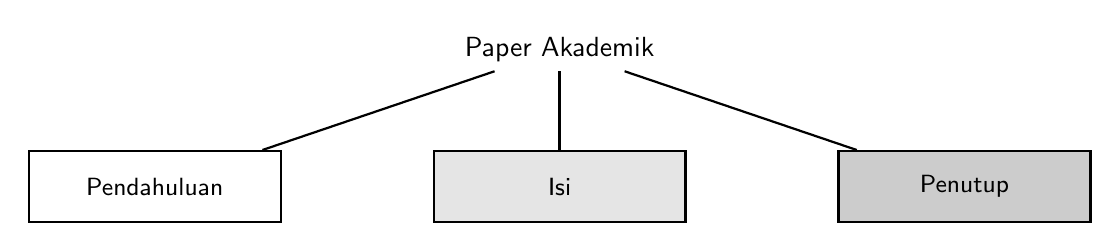
\begin{tikzpicture}[
			node distance=0.5cm and 0.8cm,
			cat/.style={rectangle, draw=black, thick, minimum width=3.2cm, minimum height=0.9cm, align=center, font=\sffamily\small},
			line/.style={draw, thick}
		]
		\node[font=\sffamily] (root) at (0, 1) {Paper Akademik};
		\node[cat, fill=white, below left=1cm and 2.2cm of root] (a) {Pendahuluan};
		\node[cat, fill=black!10, below=1cm of root] (b) {Isi};
		\node[cat, fill=black!20, below right=1cm and 2.2cm of root] (c) {Penutup};

		\draw[line] (root) -- (a);
		\draw[line] (root) -- (b);
		\draw[line] (root) -- (c);
	\end{tikzpicture}
	\caption{Hierarki tiga bagian utama paper.}
	\label{fig:hierarchy}
\end{figure}

Tiga cabang pada Gambar~\ref{fig:hierarchy} memakai tiga tingkat gradasi abu-abu untuk membedakan tanpa memakai warna. Gradasi tidak lebih gelap dari \texttt{black!30} sesuai aturan skill.

\section{Visual Tipe B: Siklus}

Siklus dipakai untuk proses yang berulang. Gambar~\ref{fig:cycle} mendemonstrasikannya pada siklus penulisan paper.

\begin{figure}[H]
	\centering
	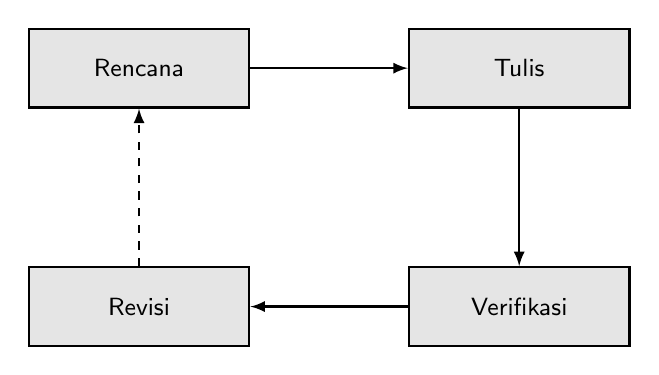
\begin{tikzpicture}[
			node distance=2cm,
			box/.style={rectangle, draw=black, thick, fill=black!10, minimum width=2.8cm, minimum height=1cm, align=center, font=\sffamily\small},
			line/.style={draw, thick, -latex}
		]
		\node[box] (plan) {Rencana};
		\node[box, right=of plan] (write) {Tulis};
		\node[box, below=of write] (verify) {Verifikasi};
		\node[box, left=of verify] (revise) {Revisi};

		\draw[line] (plan) -- (write);
		\draw[line] (write) -- (verify);
		\draw[line] (verify) -- (revise);
		\draw[line, dashed] (revise) -- (plan);
	\end{tikzpicture}
	\caption{Siklus empat tahap penulisan paper.}
	\label{fig:cycle}
\end{figure}

Garis putus-putus dari Revisi kembali ke Rencana menandakan bahwa proses tidak linear. Setelah revisi, penulis sering harus merencanakan ulang sebelum menulis lagi.

\section{Visual Tipe E: Timeline Horizontal}

Timeline dipakai untuk menunjukkan urutan waktu. Gambar~\ref{fig:timeline} mendemonstrasikannya pada evolusi skill ini.

\begin{figure}[H]
	\centering
	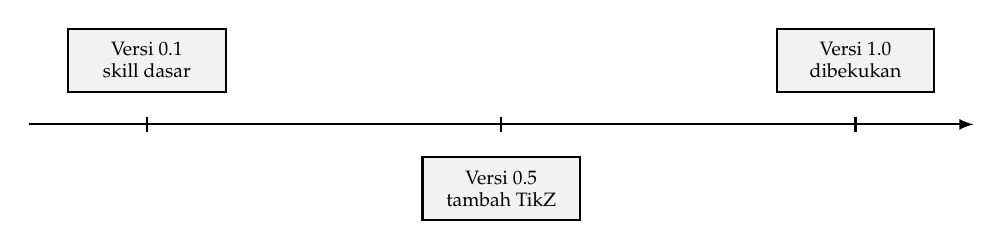
\begin{tikzpicture}[
			ev/.style={rectangle, draw=black, thick, fill=black!5, minimum width=2cm, minimum height=0.8cm, align=center, font=\scriptsize},
			line/.style={draw, thick}
		]
		\draw[line, -latex] (-6, 0) -- (6, 0);

		\draw[thick] (-4.5, 0.1) -- (-4.5, -0.1);
		\node[ev, above=0.2cm] at (-4.5, 0.2) {Versi 0.1 \\ skill dasar};

		\draw[thick] (0, 0.1) -- (0, -0.1);
		\node[ev, below=0.2cm] at (0, -0.2) {Versi 0.5 \\ tambah TikZ};

		\draw[thick] (4.5, 0.1) -- (4.5, -0.1);
		\node[ev, above=0.2cm] at (4.5, 0.2) {Versi 1.0 \\ dibekukan};
	\end{tikzpicture}
	\caption{Timeline evolusi skill.}
	\label{fig:timeline}
\end{figure}

\section{Visual Tipe F: Perbandingan Berdampingan}

Perbandingan berdampingan menampilkan dua konsep yang berlawanan secara filosofis. Gambar~\ref{fig:comparison} mendemonstrasikannya.

\begin{figure}[H]
	\centering
	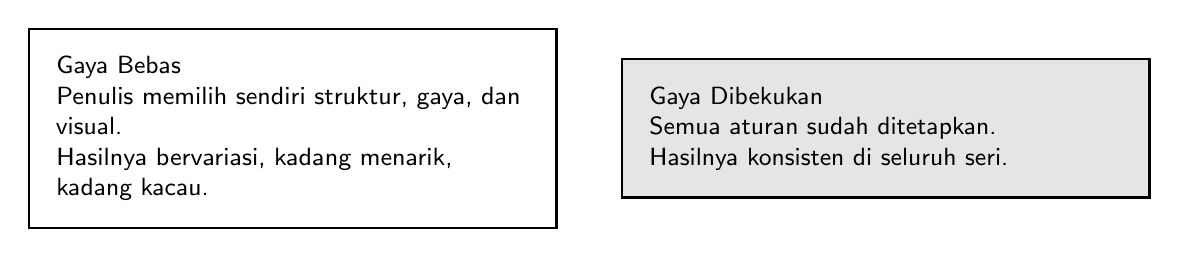
\begin{tikzpicture}[
			box/.style={rectangle, draw=black, thick, text width=6cm, align=left, font=\sffamily\small, inner sep=10pt}
		]
		\node[box, fill=white] (a) {
			Gaya Bebas \\
			Penulis memilih sendiri struktur, gaya, dan visual. \\
			Hasilnya bervariasi, kadang menarik, kadang kacau.
		};
		\node[box, fill=black!10, right=0.8cm of a] (b) {
			Gaya Dibekukan \\
			Semua aturan sudah ditetapkan. \\
			Hasilnya konsisten di seluruh seri.
		};
	\end{tikzpicture}
	\caption{Perbandingan gaya bebas dan gaya dibekukan.}
	\label{fig:comparison}
\end{figure}

\section{Visual Tipe H: Prosedur Bertahap}

Prosedur bertahap dipakai untuk menunjukkan langkah-langkah. Gambar~\ref{fig:procedure} mendemonstrasikannya pada prosedur menulis paper.

\begin{figure}[H]
	\centering
	\begin{tikzpicture}[
			step/.style={rectangle, draw=black, thick, fill=black!5, text width=9cm, align=left, minimum height=0.7cm, font=\sffamily\small, inner sep=8pt},
			line/.style={draw, thick, -latex}
		]
		\node[step] (s1) {\textbf{1.} Tentukan topik dan cakupan};
		\node[step, below=0.3cm of s1] (s2) {\textbf{2.} Rencanakan 5 sampai 12 visual};
		\node[step, below=0.3cm of s2] (s3) {\textbf{3.} Pilih analogi untuk setiap konsep};
		\node[step, below=0.3cm of s3] (s4) {\textbf{4.} Tulis bertahap per bagian};
		\node[step, below=0.3cm of s4] (s5) {\textbf{5.} Jalankan lima Quality Gates};

		\draw[line] (s1) -- (s2);
		\draw[line] (s2) -- (s3);
		\draw[line] (s3) -- (s4);
		\draw[line] (s4) -- (s5);
	\end{tikzpicture}
	\caption{Prosedur lima langkah menulis paper.}
	\label{fig:procedure}
\end{figure}

\section{Visual Tipe I: Alokasi Memori}

Alokasi memori menampilkan ukuran relatif. Gambar~\ref{fig:memory} mendemonstrasikannya pada ukuran tabel dengan primary key berbeda.

\begin{figure}[H]
	\centering
	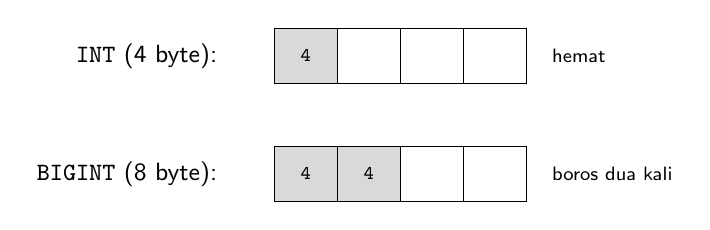
\begin{tikzpicture}[
			cell/.style={rectangle, draw=black, minimum width=0.8cm, minimum height=0.7cm, font=\ttfamily\scriptsize, align=center},
			lbl/.style={font=\sffamily\small}
		]
		\node[lbl, anchor=east] at (-1, 1.5) {\texttt{INT} (4 byte):};
		\node[cell, fill=black!15] (a1) at (0, 1.5) {4};
		\node[cell, fill=white]    (a2) at (0.8, 1.5) { };
		\node[cell, fill=white]    (a3) at (1.6, 1.5) { };
		\node[cell, fill=white]    (a4) at (2.4, 1.5) { };
		\node[font=\scriptsize\sffamily, right=0.2cm of a4] {hemat};

		\node[lbl, anchor=east] at (-1, 0) {\texttt{BIGINT} (8 byte):};
		\node[cell, fill=black!15] (b1) at (0, 0) {4};
		\node[cell, fill=black!15] (b2) at (0.8, 0) {4};
		\node[cell, fill=white]    (b3) at (1.6, 0) { };
		\node[cell, fill=white]    (b4) at (2.4, 0) { };
		\node[font=\scriptsize\sffamily, right=0.2cm of b4] {boros dua kali};
	\end{tikzpicture}
	\caption{Alokasi memori untuk primary key 4 byte dan 8 byte.}
	\label{fig:memory}
\end{figure}

\section{Pola Kode dan Tabel}

\subsection{Blok Kode Perintah}

Setiap perintah yang diajarkan memakai gaya \texttt{code}.

\begin{lstlisting}[style=code]
CREATE TABLE contoh (
    id BIGINT UNSIGNED DEFAULT (UUID_SHORT()) PRIMARY KEY,
    nama VARCHAR(100) NOT NULL
);
\end{lstlisting}

\subsection{Blok Kode Keluaran}

Keluaran perintah memakai gaya \texttt{out}.

\begin{lstlisting}[style=out]
+-------+---------------+
| Field | Type          |
+-------+---------------+
| id    | bigint(20)    |
| nama  | varchar(100)  |
+-------+---------------+
2 rows in set
\end{lstlisting}

\subsection{Tabel Booktabs}

Semua tabel memakai \texttt{booktabs}.

\begin{table}[H]
	\centering
	\caption{Contoh tabel booktabs.}
	\label{tab:example}
	\small
	\begin{tabular}{l l l}
		\toprule
		Kolom 1 & Kolom 2 & Kolom 3 \\
		\midrule
		baris 1 & isi 1   & isi 2   \\
		baris 2 & isi 3   & isi 4   \\
		baris 3 & isi 5   & isi 6   \\
		\bottomrule
	\end{tabular}
\end{table}

Perhatikan tidak ada garis vertikal, tidak ada warna latar, dan header memakai teks biasa tanpa bold.

\section{Studi Kasus: Menyusun Satu Paper}

\subsection{Langkah 1: Pahami Permintaan}

Sebelum menulis, baca permintaan sampai habis. Tentukan topik, cakupan, tingkat kedalaman, dan audiens.

\subsection{Langkah 2: Rencanakan Visual}

Daftar 5 sampai 12 visual. Untuk setiap visual, tentukan tipe diagramnya.

\subsection{Langkah 3: Pilih Analogi}

Satu analogi per konsep. Jangan pakai analogi yang sama dua kali.

\subsection{Langkah 4: Tulis Pendahuluan}

Buka dengan analogi, jelaskan tesis, akhiri dengan peta bagian.

\subsection{Langkah 5: Tulis Bagian Konsep}

Setiap subbagian menjawab mengapa, bukan hanya apa.

\subsection{Langkah 6: Sisipkan Visual}

Setiap 2 sampai 3 subbagian diselingi satu diagram.

\subsection{Langkah 7: Tulis Studi Kasus}

Minimal 8 langkah. Setiap langkah punya blok kode.

\subsection{Langkah 8: Verifikasi}

Jalankan lima Quality Gates: kompilasi, gaya, struktur, visual, terminologi.

\section{Kesalahan Umum dan Cara Menghindarinya}

\begin{table}[H]
	\centering
	\caption{Kesalahan umum pada penulisan paper dengan skill ini.}
	\label{tab:mistakes}
	\footnotesize
	\begin{tabularx}{\textwidth}{l X X}
		\toprule
		Kesalahan                                                          & Akibat                    & Perbaikan                                       \\
		\midrule
		komentar \texttt{\%} tertinggal                                    & melanggar aturan skill    & hapus semua komentar                            \\
		warna eksplisit di TikZ                                            & melanggar palet           & pakai \texttt{black!N} saja                     \\
		\texttt{\textbackslash rowcolor} di tabel                          & tidak konsisten           & pakai \texttt{booktabs} tanpa warna             \\
		blok kode gaya campuran                                            & tampilan tidak konsisten  & pilih \texttt{code} atau \texttt{out} saja      \\
		\texttt{\textbackslash hline} di tabel                             & tidak booktabs            & pakai \texttt{\textbackslash midrule}           \\
		diagram tanpa label                                                & tidak bisa dirujuk        & tambah \texttt{\textbackslash label\{fig:...\}} \\
		placeholder tertinggal                                             & makalah tidak siap        & cari "TODO" sebelum submit                      \\
		heading tak konsisten                                              & struktur kacau            & patuhi resep Bagian 8                           \\
		\texttt{\textbackslash today} di luar \texttt{\textbackslash date} & tanggal salah konteks     & biarkan hanya di \texttt{\textbackslash date}   \\
		\texttt{\textbackslash textbf\{\textbackslash textit\{...\}\}}     & bold dan italic bertumpuk & pilih salah satu                                \\
		\bottomrule
	\end{tabularx}
\end{table}

\section{Lembar Rujukan Cepat}

\begin{table}[H]
	\centering
	\caption{Rujukan cepat pola LaTeX pada skill ini.}
	\label{tab:cheat}
	\footnotesize
	\begin{tabularx}{\textwidth}{l X}
		\toprule
		Kebutuhan        & Pola                                                                \\
		\midrule
		preamble         & sesuai Bagian 2, verbatim                                           \\
		judul            & \texttt{\textbackslash title\{\textbackslash vspace\{-1.5cm\}...\}} \\
		abstract         & environment \texttt{abstract} yang sudah didefinisikan              \\
		kode perintah    & \texttt{\textbackslash begin\{lstlisting\}[style=code]}             \\
		kode keluaran    & \texttt{\textbackslash begin\{lstlisting\}[style=out]}              \\
		tabel standar    & \texttt{booktabs} dengan \texttt{tabular}                           \\
		tabel panjang    & \texttt{booktabs} dengan \texttt{tabularx}                          \\
		diagram          & \texttt{tikzpicture} dengan gaya inline                             \\
		gradasi abu      & \texttt{black!5} sampai \texttt{black!30}                           \\
		referensi inline & \texttt{\textbackslash cite\{kunci\}}                               \\
		referensi daftar & \texttt{\textbackslash bibitem\{kunci\}}                            \\
		referensi Gambar & \texttt{Gambar\textasciitilde\textbackslash ref\{fig:...\}}         \\
		referensi Tabel  & \texttt{Tabel\textasciitilde\textbackslash ref\{tab:...\}}          \\
		halaman baru     & \texttt{\textbackslash newpage} sebelum Referensi                   \\
		penutup          & \texttt{\textbackslash end\{document\}}                             \\
		\bottomrule
	\end{tabularx}
\end{table}

\section{Kesimpulan}

Makalah ini mendemonstrasikan seluruh pola gaya yang dibekukan dalam skill. Tiga prinsip penutup:

\begin{enumerate}
	\item Skill adalah kontrak, bukan saran. Setiap aturan di dalamnya berlaku mutlak, mulai dari preamble hingga penutup.
	\item Visual adalah penjelas, bukan hiasan. Setiap diagram harus menerangkan konsep, bukan sekadar mengisi ruang.
	\item Konsistensi mengalahkan kreativitas. Satu gaya yang dipatuhi di seluruh seri menghasilkan makalah yang terasa seperti jurnal, bukan blog.
\end{enumerate}

Pembaca yang telah memahami makalah ini siap menerapkan skill pada topik apa pun, dari basis data hingga ilmu sosial.

\newpage
\section*{Referensi}
\addcontentsline{toc}{section}{Referensi}

\begin{thebibliography}{99}

	\bibitem{lamport}
	Lamport, L. (1994).
	\textit{LaTeX: A Document Preparation System} (2nd ed.).
	Addison-Wesley.

	\bibitem{mittelbach}
	Mittelbach, F., \& Goossens, M. (2004).
	\textit{The LaTeX Companion} (2nd ed.).
	Addison-Wesley.

	\bibitem{silberschatz}
	Silberschatz, A., Korth, H. F., \& Sudarshan, S. (2019).
	\textit{Database System Concepts} (7th ed.).
	McGraw-Hill Education.

	\bibitem{klabnik}
	Klabnik, S., \& Nichols, C. (2019).
	\textit{The Rust Programming Language}.
	No Starch Press.

	\bibitem{mariadb-ddl}
	MariaDB Foundation. (2026).
	\textit{SQL Statements --- CREATE TABLE, ALTER TABLE,
		DROP TABLE}.
	MariaDB Knowledge Base.
	\texttt{https://mariadb.com/kb/en/sql-statements/}

	\bibitem{tikz}
	Tantau, T. (2024).
	\textit{The TikZ and PGF Packages}.
	\texttt{https://tikz.dev/}

\end{thebibliography}

\end{document}
